\section{Phase de conceptualisation}
\subsection{Produit imaginé}
Pour répondre à tous les besoins de la cliente, nous avons imaginé un produit simple et facile à utiliser. Cas d'utilisation :
\begin{itemize}
    \item Installation simple par branchement des capteurs, puis les aimanter sous le trampoline.
    \item Appuyer sur le bouton du boitier principal pendant un saut pour lancer les mesures.
    \item Vérifier les mesures sur l'écran.
    \item Après dix sauts, le score s'affiche sur l'écran
    \item Une fois les différentes mesures faites, appuyer sur le bouton Wifi, puis se connecter au wifi et accéder au site internet.
    \item Consulter les mesures en détail sur le site internet, télécharger les données sous format Microsoft Excel.
    \item Appuyer à nouveau sur le bouton Wifi pour refaire des mesures de temps.
\end{itemize}

%Les composants :
\subsection{Choix des composants}
Les déférents composants ont été choisis en fonction de leurs couts, de leurs disponibilités et leurs facilités d'utilisation.
\paragraph{Capteur :}
Le composant le plus onéreux. Il est crucial pour la fiabilité des mesures. Nous avons choisi des capteurs laser. Le projet ne partant de rien, nous avons préféré prendre des capteurs de premiers prix. C'est un capteur de type NPN, ayant une distance maximum de 20 mètres et fonctionnant avec des tensions allant de 6 à 20V.

\paragraph{Microcontrolleur :}
Il fallait une cible très accessible avec un module Wifi. Le NodeMCU correspond parfaitement à nos besoins : il possède un module Wifi, fonctionne avec les bibliothèques Arduino, possède un mémoire flash de quatre mégaoctets et à une horloge de 80Mz permettant une lecture rapide des entrées.

\paragraph{Ecran :}
Nous avons choisi un  écran Oled, fonctionnant uniquement en I2C, pour la facilité d'utilisation et la lisibilité de l'image en pleine lumière. Il est petit et peut facilement être remplacé pour un plus grand modèle si besoin est.

\paragraph{Alimentation :}
Nous avons préféré utiliser des modules peu puissants. c'est pour cela que nous avons pris deux transformateurs 5V, 2A. Ces tensions sont suffisamment faibles pour ne pas être dangereuses en cas d'électrocution ou en cas de cours circuit. Ils sont ce dont nous avons besoin pour tester, mais devront être augmentés pour la partie émetteur laser, car une tentions de minimum 6V est demandé. Nous avons fait fonctionner le capteur sous 9V et sous 5V. 5V est faible, mais suffisant, car la distance sous le trampoline est courte. 9V est optimal, mais le rayon laser est plus puissant et du coup plus dangereux.

\paragraph{Connectique :}
Nous avons pris une connectique très accessible. Pour la partie alimentation, nous avons pris des connecteurs $5.5mm * 2.1mm$. Pour la partie récepteur, il nous fallait des connecteurs 3 pins. Nous avons choisi de prendre des connecteurs Jack $6.3mm$.

\subsection{Architecture logicielle}
La partie logiciel nous permet de mettre en relation tous les composants. La fonction première du produit étant de chronométrer, nous comptions utiliser l'horloge interne du microcontrôleur pour faire cela. Comme dit précédemment, l'horloge interne tourne à une vitesse de 80MHz (soit à 12,5 nanosecondes d'intervalle). Pour ne pas avoir de perte de précision dans les données, nous avons choisi de stocker toutes les mesures en microsecondes puisque c'est ce qui est utilisé en interne par la bibliothèque Arduino. La précision recherchée étant la milliseconde, cela nous convenait. Les valeurs sont forcément positives, nous avons donc utilisé des nombres non signés. Le microcontrôleur étant construit sur une architecture à 32 bits, stocker les mesures sur des nombres 32bis était le plus pertinent, sachant que la valeur maximum d'un temps en microsecondes non signé sur 32 bits revient à environ 71 minutes. Dans le cas où une valeur dépasserait la maximale, le compteur recommencerait à zéro. 

Ci-dessous le diagramme de classe alors imaginé pour la partie logiciel.

\begin{center}
  \makebox[\textwidth]{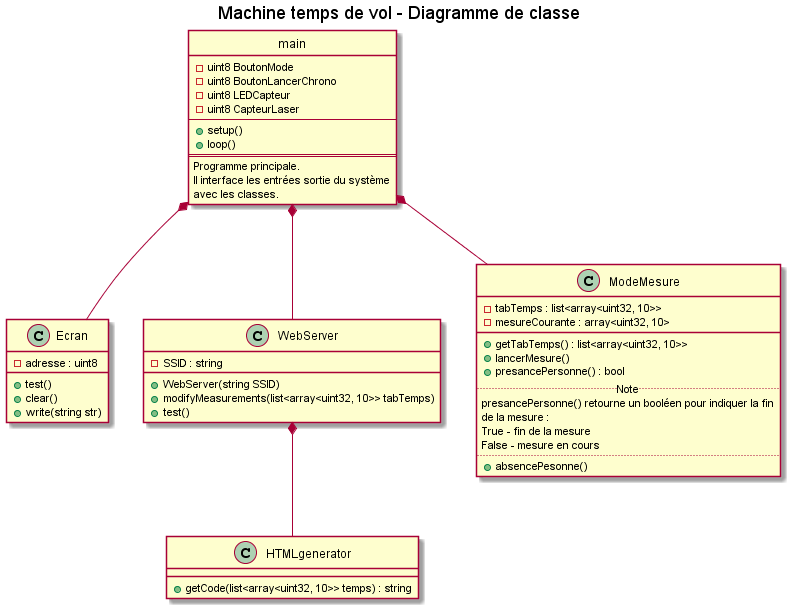
\includegraphics[width=15cm]{photoAlex/diagrammeDeClasse_Ancien.png}}
  
  Diagramme de classe initialement prévu pour la partie logiciel.
\end{center}
